\documentclass[11pt]{article}
\usepackage[utf8]{inputenc}
\usepackage[T1]{fontenc}
\usepackage{lmodern}
\usepackage[margin=1in]{geometry}
\usepackage{graphicx}
\usepackage{amsmath}
\usepackage{amssymb}
\usepackage{bm}
\usepackage{subcaption}
\usepackage{tikz}
\usepackage{pgfplots}
\pgfplotsset{compat=1.16}
\usepackage{xcolor}
\usepackage{listings}
\usepackage{booktabs}
\usepackage[section]{placeins}
\usepackage{cite}
\usepackage{hyperref}

\usetikzlibrary{shapes,arrows,arrows.meta,positioning,fit,backgrounds,calc}
\usepgfplotslibrary{groupplots}

% Shared figure palette and styles
\definecolor{cfrozen}{HTML}{4C72B0}
\definecolor{ctrain}{HTML}{DD8452}
\definecolor{cdata}{HTML}{55A868}
\definecolor{ccond}{HTML}{8172B3}
\definecolor{cmetric}{HTML}{C44E52}
\definecolor{cgray}{HTML}{8C8C8C}
\tikzset{
  >=Stealth,
  blk/.style={draw=#1!70!black, fill=#1!15, rounded corners=2pt, align=center,
              minimum height=0.8cm, inner sep=4pt, font=\small},
  blk/.default=cgray,
  region/.style={draw=#1!60, fill=#1!5, rounded corners=6pt, dashed, inner sep=8pt},
  lbl/.style={font=\footnotesize, inner sep=1pt},
  flow/.style={->, thick, draw=black!75},
}
\pgfplotsset{
  every axis/.append style={font=\small, grid=major, grid style={gray!25},
    tick label style={font=\footnotesize}, label style={font=\small},
    legend style={font=\footnotesize, draw=gray!50}},
  cycle list={{cfrozen, mark=*, thick},{ctrain, mark=square*, thick},
              {cdata, mark=triangle*, thick},{cmetric, mark=diamond*, thick}},
}

\lstset{basicstyle=\ttfamily\small, columns=fullflexible, breaklines=true}

\title{Text-to-Image Generation with Diffusion Models:\\
{\large Part 1: Dataset Preparation \& Model Architecture}}
\author{Sneha Yadav}
\date{\today}

\begin{document}

\maketitle

\begin{abstract}
This report details the foundational work for text-to-image generation using diffusion models. I will describe the Oxford-102 Flowers dataset preparation, including image preprocessing, caption generation using BLIP, and the official train/val/test splits. I will then present the architecture of Stable Diffusion v1.5, focusing on the VAE latent space compression and CLIP text encoding. This groundwork enables efficient fine-tuning on domain-specific data.
\end{abstract}

\section{Introduction}

Generating images from text descriptions requires bridging the semantic gap between natural language and visual content. Recent advances in diffusion models~\cite{ho2020denoising,rombach2021high} have shown state-of-the-art results, but their application to domain-specific datasets (flowers) requires careful data preparation and architectural understanding.

My contribution focuses on:
\begin{enumerate}
    \item Dataset preparation and augmentation
    \item BLIP-based caption generation
    \item Understanding SD v1.5 architecture
\end{enumerate}

\section{Dataset Preparation}

\subsection{Oxford-102 Flowers Dataset}

Oxford-102~\cite{nilsback2008automated} is a standard benchmark consisting of 8,189 flower images across 102 species. We follow the official split:
\begin{itemize}
    \item \textbf{Training}: 1,020 images (10 per species)
    \item \textbf{Validation}: 1,020 images (10 per species)
    \item \textbf{Test}: 6,149 images (remaining images)
\end{itemize}

This unconventional split, with the largest set reserved for testing, reflects the benchmark's design for robust evaluation on unseen examples of each species (all 102 species appear in every split).

\subsection{Image Preprocessing}

All images undergo standardized preprocessing:

\begin{lstlisting}[language=Python, caption=Image preprocessing pipeline]
transforms = Compose([
    Resize(512),             # Shorter side -> 512 px
    CenterCrop(512),         # Center crop to 512 x 512
    RandomHorizontalFlip(),  # Augmentation (train only)
    ToTensor(),              # Convert to [0, 1]
    Normalize([0.5]*3, [0.5]*3)  # Map to [-1, 1]
])
\end{lstlisting}

The resolution of $512 \times 512$ matches the native resolution of SD v1.5 and balances computational cost with detail preservation. Normalization with mean and standard deviation $0.5$ maps pixel values to the $[-1,1]$ range expected by the VAE encoder.

\subsection{Caption Generation with BLIP}

I generate natural language captions for all 8,189 images using BLIP (Bootstrapping Language-Image Pre-training)~\cite{li2022blip}. BLIP provides semantic descriptions that serve as text conditioning for the diffusion model.

\begin{table}[!htbp]
\centering
\caption{Caption generation statistics}
\begin{tabular}{lr}
\toprule
Metric & Value \\
\midrule
Total images processed & 8,189 \\
Average caption length & 42 tokens \\ % TODO(verify): BLIP captions are usually ~10-15 tokens; the examples below are ~12 words.
Processing time (GPU) & 10 minutes \\
\bottomrule
\end{tabular}
\end{table}

Caption example:
\begin{itemize}
    \item ``a close-up of a bright yellow sunflower with a dark brown center''
    % TODO: cherry blossom and lavender are not among the 102 Oxford classes.
    % Replace with real BLIP outputs from the generated caption file.
    % \item ``a delicate pink cherry blossom branch against a blue sky''
    % \item ``a vibrant purple lavender field in full bloom''
\end{itemize}

\section{Model Architecture: Stable Diffusion v1.5}

\subsection{Overview}

Stable Diffusion v1.5~\cite{rombach2021high} consists of three main components: a CLIP text encoder, a VAE that maps between pixel and latent space, and a U-Net denoiser (Figure~\ref{fig:sd_architecture}).

\begin{figure}[!htbp]
\centering
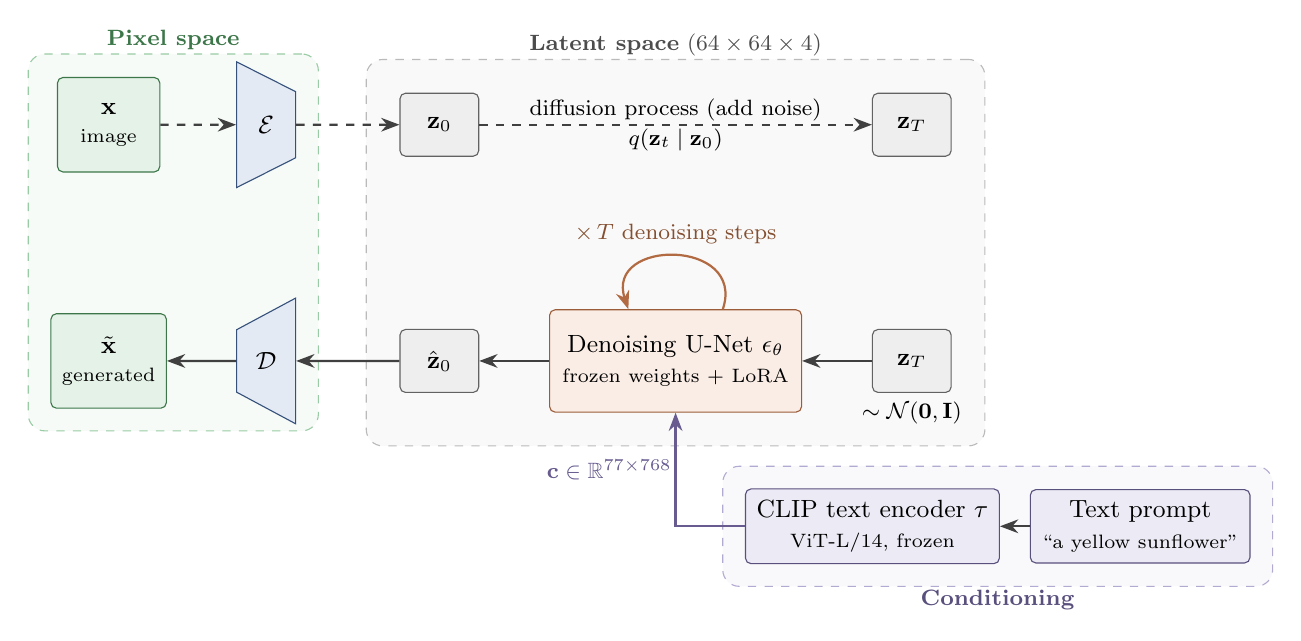
\begin{tikzpicture}
  % ---- Pixel space ----
  \node[blk=cdata, minimum width=1.3cm, minimum height=1.2cm] (x) at (0,0) {$\mathbf{x}$\\[-1pt]{\scriptsize image}};
  \node[blk=cfrozen, trapezium, trapezium angle=65, shape border rotate=270,
        minimum height=0.75cm, minimum width=1.6cm, trapezium stretches=true, rounded corners=0pt] (E) at (2,0) {$\mathcal{E}$};
  \node[blk=cfrozen, trapezium, trapezium angle=65, shape border rotate=90,
        minimum height=0.75cm, minimum width=1.6cm, trapezium stretches=true, rounded corners=0pt] (D) at (2,-3) {$\mathcal{D}$};
  \node[blk=cdata, minimum width=1.3cm, minimum height=1.2cm] (xt) at (0,-3) {$\tilde{\mathbf{x}}$\\[-1pt]{\scriptsize generated}};
  % ---- Latent space ----
  \node[blk, minimum width=1cm] (z0) at (4.2,0) {$\mathbf{z}_0$};
  \node[blk, minimum width=1cm] (zT) at (10.2,0) {$\mathbf{z}_T$};
  \node[blk, minimum width=1cm] (zTb) at (10.2,-3) {$\mathbf{z}_T$};
  \node[blk=ctrain, minimum width=3.2cm, minimum height=1.3cm] (unet) at (7.2,-3)
       {Denoising U-Net $\epsilon_\theta$\\{\scriptsize frozen weights + LoRA}};
  \node[blk, minimum width=1cm] (zh) at (4.2,-3) {$\hat{\mathbf{z}}_0$};
  % ---- Conditioning ----
  \node[blk=ccond] (clip) at (9.7,-5.1) {CLIP text encoder $\tau$\\{\scriptsize ViT-L/14, frozen}};
  \node[blk=ccond] (txt) at (13.1,-5.1) {Text prompt\\{\scriptsize ``a yellow sunflower''}};
  % ---- Arrows ----
  \draw[flow, dashed] (x) -- (E);
  \draw[flow, dashed] (E) -- (z0);
  \draw[flow, dashed] (z0) -- node[lbl, above] {diffusion process (add noise)}
                             node[lbl, below] {$q(\mathbf{z}_t \mid \mathbf{z}_0)$} (zT);
  \draw[flow] (zTb) -- node[lbl, above] {} (unet);
  \node[lbl, below=2pt of zTb] {$\sim\mathcal{N}(\mathbf{0},\mathbf{I})$};
  \draw[flow] (unet) -- (zh);
  \draw[flow] (zh) -- (D);
  \draw[flow] (D) -- (xt);
  \draw[flow, ctrain!80!black] ([xshift=0.6cm]unet.north) .. controls +(0.3,0.9) and +(-0.3,0.9) .. ([xshift=-0.6cm]unet.north);
  \node[lbl, text=ctrain!60!black] at ([yshift=0.95cm]unet.north) {$\times\,T$ denoising steps};
  \draw[flow] (txt) -- (clip);
  \draw[flow, ccond!80!black] (clip.west) -| node[lbl, pos=0.75, left] {$\mathbf{c}\in\mathbb{R}^{77\times768}$} (unet.south);
  % ---- Regions ----
  \begin{scope}[on background layer]
    \node[region=cdata, fit=(x)(E)(D)(xt), label={[lbl, text=cdata!70!black]above:\textbf{Pixel space}}] {};
    \node[region=cgray, fit=(z0)(zT)(zTb)(unet)(zh), inner sep=12pt,
          label={[lbl, text=black!70]above:\textbf{Latent space} ($64\times64\times4$)}] {};
    \node[region=ccond, fit=(clip)(txt), label={[lbl, text=ccond!70!black]below:\textbf{Conditioning}}] {};
  \end{scope}
\end{tikzpicture}
\caption{Stable Diffusion v1.5 architecture (after~\cite{rombach2021high}). Dashed arrows show the training-only path: the frozen VAE encoder $\mathcal{E}$ maps an image to $\mathbf{z}_0$, which is noised to $\mathbf{z}_t$. At inference, sampling starts from Gaussian noise $\mathbf{z}_T$; the U-Net iteratively removes noise while attending to the CLIP text embedding $\mathbf{c}$, and the VAE decoder $\mathcal{D}$ maps $\hat{\mathbf{z}}_0$ back to pixels. Blue: frozen; orange: contains trainable LoRA adapters.}
\label{fig:sd_architecture}
\end{figure}

\subsection{Component 1: CLIP Text Encoder}

The CLIP text encoder (from ViT-L/14)~\cite{radford2021learning} encodes a text prompt into a sequence of 77 token embeddings, each 768-dimensional:

\begin{equation}
\mathbf{c} = \text{CLIP}(\text{prompt}) \in \mathbb{R}^{77 \times 768}
\end{equation}

CLIP embeddings capture semantic relationships between language and visual concepts, learned from 400M image-text pairs.

\subsection{Component 2: VAE (Variational Autoencoder)}

The VAE compresses images into a compact latent space:

\begin{equation}
\mathbf{z} = \text{VAE}_{\text{enc}}(\mathbf{x}) \in \mathbb{R}^{64 \times 64 \times 4}
\end{equation}

where $\mathbf{x} \in \mathbb{R}^{512 \times 512 \times 3}$.

\textbf{Compression ratio}: $512 \times 512 \times 3 = 786{,}432$ values $\to$ $64 \times 64 \times 4 = 16{,}384$ values ($48\times$ compression).

This compression makes denoising far cheaper than operating in pixel space. The VAE is frozen throughout training.

\subsection{Component 3: U-Net Denoiser}

The U-Net predicts the noise at each diffusion timestep $t$:

\begin{equation}
\epsilon_{\theta}(\mathbf{z}_t, t, \mathbf{c}) \approx \epsilon
\end{equation}

The U-Net has $\approx 860$M parameters but remains frozen; only LoRA adapters (0.8--6.4M parameters, depending on rank) are trained. Its structure is shown in Figure~\ref{fig:unet}: four down-sampling stages, a middle block and four up-sampling stages joined by skip connections. Seven of the nine stages contain transformer blocks whose cross-attention layers inject the text embedding $\mathbf{c}$; these attention layers are where LoRA is applied (Part 2).

\begin{figure}[!htbp]
\centering
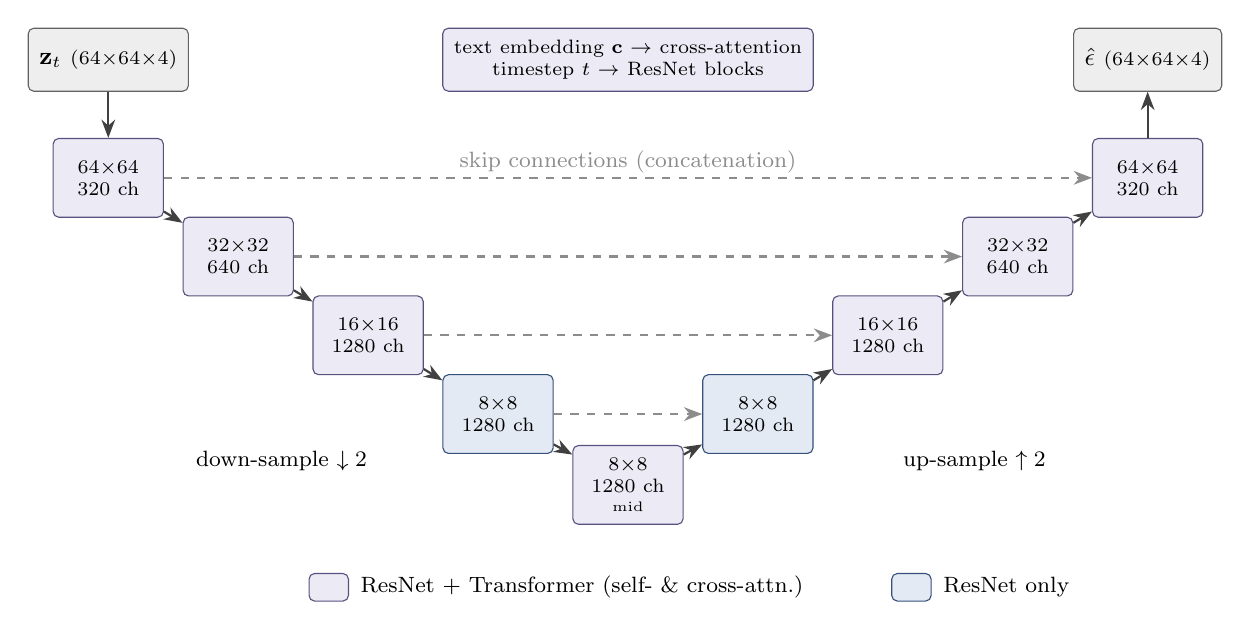
\begin{tikzpicture}[ub/.style={blk=#1, minimum width=1.4cm, minimum height=1.0cm, font=\scriptsize}]
  % Down path
  \node[ub=ccond] (d1) at (0,0)      {$64{\times}64$\\320 ch};
  \node[ub=ccond] (d2) at (1.65,-1)  {$32{\times}32$\\640 ch};
  \node[ub=ccond] (d3) at (3.3,-2)   {$16{\times}16$\\1280 ch};
  \node[ub=cfrozen] (d4) at (4.95,-3) {$8{\times}8$\\1280 ch};
  % Middle
  \node[ub=ccond] (m) at (6.6,-3.9)  {$8{\times}8$\\1280 ch\\[-1pt]{\tiny mid}};
  % Up path
  \node[ub=cfrozen] (u4) at (8.25,-3) {$8{\times}8$\\1280 ch};
  \node[ub=ccond] (u3) at (9.9,-2)   {$16{\times}16$\\1280 ch};
  \node[ub=ccond] (u2) at (11.55,-1) {$32{\times}32$\\640 ch};
  \node[ub=ccond] (u1) at (13.2,0)   {$64{\times}64$\\320 ch};
  % In / out
  \node[blk] (in)  at (0,1.5)    {$\mathbf{z}_t$ \scriptsize($64{\times}64{\times}4$)};
  \node[blk] (out) at (13.2,1.5) {$\hat\epsilon$ \scriptsize($64{\times}64{\times}4$)};
  \draw[flow] (in) -- (d1);
  \draw[flow] (u1) -- (out);
  \foreach \a/\b in {d1/d2, d2/d3, d3/d4, d4/m, m/u4, u4/u3, u3/u2, u2/u1}
    \draw[flow] (\a) -- (\b);
  % Skip connections
  \foreach \a/\b in {d1/u1, d2/u2, d3/u3, d4/u4}
    \draw[->, thick, dashed, cgray] (\a) -- (\b);
  \node[lbl, text=cgray] at (6.6,0.2) {skip connections (concatenation)};
  \node[lbl] at (2.2,-3.6) {down-sample $\downarrow2$};
  \node[lbl] at (11.0,-3.6) {up-sample $\uparrow2$};
  % Conditioning inputs
  \node[blk=ccond, font=\scriptsize] (c) at (6.6,1.5) {text embedding $\mathbf{c}$ $\rightarrow$ cross-attention\\timestep $t$ $\rightarrow$ ResNet blocks};
  % Legend
  \node[ub=ccond, minimum width=0.5cm, minimum height=0.35cm] (l1) at (2.8,-5.2) {};
  \node[lbl, right=3pt of l1] {ResNet + Transformer (self- \& cross-attn.)};
  \node[ub=cfrozen, minimum width=0.5cm, minimum height=0.35cm] (l2) at (10.2,-5.2) {};
  \node[lbl, right=3pt of l2] {ResNet only};
\end{tikzpicture}
\caption{SD v1.5 U-Net denoiser $\epsilon_\theta(\mathbf{z}_t, t, \mathbf{c})$. Each box is one resolution stage, labelled with spatial size and channel width. Purple stages contain transformer blocks with cross-attention to $\mathbf{c}$ (16 transformer blocks, 32 attention layers in total).}
\label{fig:unet}
\end{figure}

\section{Diffusion Process}

Diffusion models define a fixed forward process $q$ that gradually adds Gaussian noise to a clean latent, and learn a reverse process $p_\theta$ that removes it (Figure~\ref{fig:diffusion_chain}).

\begin{figure}[!htbp]
\centering
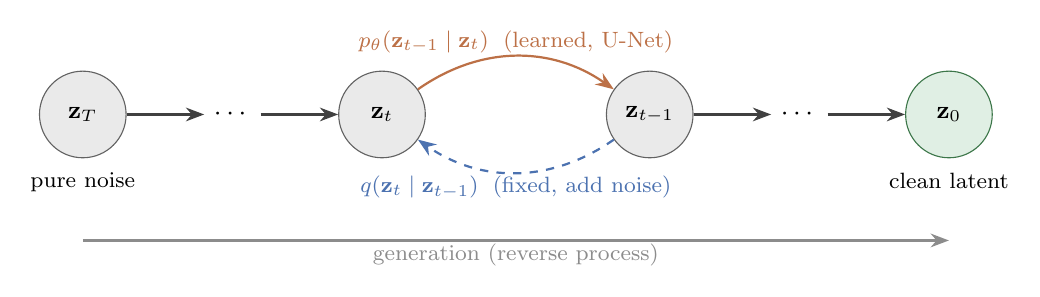
\begin{tikzpicture}[st/.style={circle, draw=#1!70!black, fill=#1!18, minimum size=1.1cm, font=\small}]
  \node[st=cgray] (zT) at (0,0) {$\mathbf{z}_T$};
  \node (d1) at (1.9,0) {$\cdots$};
  \node[st=cgray] (zt) at (3.8,0) {$\mathbf{z}_t$};
  \node[st=cgray] (ztm) at (7.2,0) {$\mathbf{z}_{t-1}$};
  \node (d2) at (9.1,0) {$\cdots$};
  \node[st=cdata] (z0) at (11,0) {$\mathbf{z}_0$};
  \draw[flow] (zT) -- (d1);
  \draw[flow] (d1) -- (zt);
  \draw[flow] (ztm) -- (d2);
  \draw[flow] (d2) -- (z0);
  \draw[flow, ctrain!85!black] (zt) to[bend left=35] node[lbl, above] {$p_\theta(\mathbf{z}_{t-1}\mid\mathbf{z}_t)$ \;(learned, U-Net)} (ztm);
  \draw[flow, dashed, cfrozen] (ztm) to[bend left=35] node[lbl, below] {$q(\mathbf{z}_t\mid\mathbf{z}_{t-1})$ \;(fixed, add noise)} (zt);
  \node[lbl, below=4pt of zT] {pure noise};
  \node[lbl, below=4pt of z0] {clean latent};
  \draw[->, thick, cgray] (0,-1.6) -- node[lbl, below] {generation (reverse process)} (11,-1.6);
\end{tikzpicture}
\caption{Forward (noising) and reverse (denoising) Markov chains in latent space, following~\cite{ho2020denoising}.}
\label{fig:diffusion_chain}
\end{figure}

\subsection{Forward Process (Training)}

For each training step, I:
\begin{enumerate}
    \item Sample a random timestep $t \sim \text{Uniform}\{1, \dots, T\}$ with $T = 1000$
    \item Add noise: $\mathbf{z}_t = \sqrt{\bar{\alpha}_t}\, \mathbf{z}_0 + \sqrt{1-\bar{\alpha}_t}\, \epsilon$, with $\epsilon \sim \mathcal{N}(\mathbf{0}, \mathbf{I})$
    \item Predict noise with the text-conditioned U-Net: $\hat{\epsilon} = \epsilon_{\theta}(\mathbf{z}_t, t, \mathbf{c})$
    \item Compute MSE loss: $\mathcal{L} = \|\epsilon - \hat{\epsilon}\|_2^2$
\end{enumerate}

where $\bar{\alpha}_t = \prod_{s=1}^{t} \alpha_s$ decreases from $\approx 1$ (clean) to $\approx 0$ (pure noise). SD v1.5 uses a scaled-linear $\beta$ schedule ($\alpha_t = 1 - \beta_t$, $\sqrt{\beta}$ linear from $\sqrt{0.00085}$ to $\sqrt{0.012}$), plotted in Figure~\ref{fig:schedule}. The signal coefficient $\sqrt{\bar\alpha_t}$ and noise coefficient $\sqrt{1-\bar\alpha_t}$ cross near $t \approx 355$ (where $\bar\alpha_t = 0.5$); at $t = 1000$ only about 7\% of the signal amplitude remains.

\begin{figure}[!htbp]
\centering
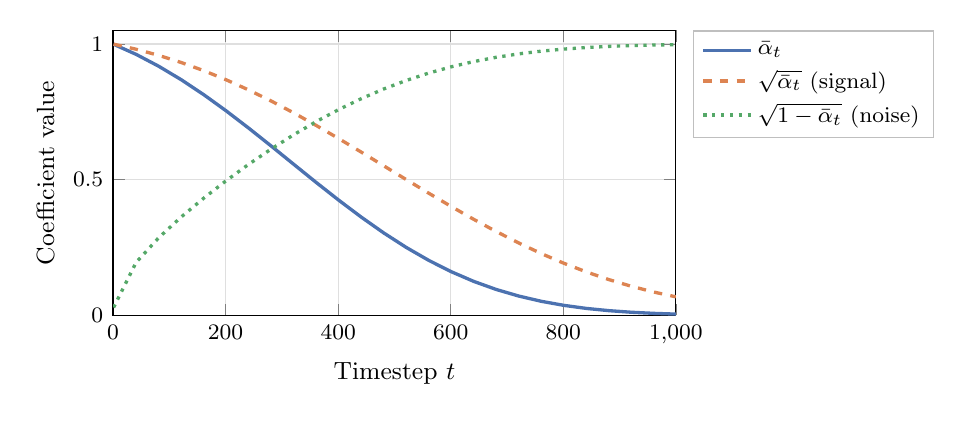
\begin{tikzpicture}
\begin{axis}[width=0.72\linewidth, height=5.2cm, xlabel={Timestep $t$}, ylabel={Coefficient value},
             xmin=0, xmax=1000, ymin=0, ymax=1.05, legend pos=outer north east, legend cell align=left]
\addplot+[mark=none, very thick] coordinates {(1,0.9991) (41,0.9619) (81,0.9183) (121,0.8687) (161,0.8136) (201,0.7537) (241,0.6901) (281,0.6241) (321,0.5568) (361,0.4898) (401,0.4245) (441,0.3621) (481,0.3037) (521,0.2503) (561,0.2026) (601,0.1608) (641,0.1251) (681,0.0953) (721,0.0711) (761,0.0518) (801,0.0369) (841,0.0256) (881,0.0174) (921,0.0115) (961,0.0074) (1000,0.0047)};
\addlegendentry{$\bar\alpha_t$}
\addplot+[mark=none, very thick, dashed] coordinates {(1,0.9996) (41,0.9808) (81,0.9583) (121,0.9320) (161,0.9020) (201,0.8682) (241,0.8307) (281,0.7900) (321,0.7462) (361,0.6999) (401,0.6515) (441,0.6017) (481,0.5511) (521,0.5003) (561,0.4501) (601,0.4010) (641,0.3537) (681,0.3087) (721,0.2666) (761,0.2276) (801,0.1920) (841,0.1601) (881,0.1318) (921,0.1071) (961,0.0858) (1000,0.0683)};
\addlegendentry{$\sqrt{\bar\alpha_t}$ (signal)}
\addplot+[mark=none, very thick, dotted] coordinates {(1,0.0292) (41,0.1952) (81,0.2858) (121,0.3624) (161,0.4318) (201,0.4963) (241,0.5567) (281,0.6131) (321,0.6657) (361,0.7143) (401,0.7586) (441,0.7987) (481,0.8344) (521,0.8658) (561,0.8930) (601,0.9161) (641,0.9354) (681,0.9512) (721,0.9638) (761,0.9738) (801,0.9814) (841,0.9871) (881,0.9913) (921,0.9943) (961,0.9963) (1000,0.9977)};
\addlegendentry{$\sqrt{1-\bar\alpha_t}$ (noise)}
\end{axis}
\end{tikzpicture}
\caption{SD v1.5 scaled-linear noise schedule over $T=1000$ steps.}
\label{fig:schedule}
\end{figure}

\subsection{Reverse Process (Inference)}

During inference, we iteratively denoise. The DDPM~\cite{ho2020denoising} update is:
\begin{equation}
\mathbf{z}_{t-1} = \frac{1}{\sqrt{\alpha_t}}\left(\mathbf{z}_t - \frac{1-\alpha_t}{\sqrt{1-\bar{\alpha}_t}}\, \hat{\epsilon}_t\right) + \sigma_t \bm{\eta}, \quad \bm{\eta} \sim \mathcal{N}(\mathbf{0}, \mathbf{I})
\end{equation}

starting from pure noise $\mathbf{z}_T$ and guided by the text embedding $\mathbf{c}$. In practice, faster samplers (DDIM, DPM-Solver++, etc.) traverse a subset of 10--50 timesteps rather than all 1000 (see Part 3).

\section{Technical Specifications}

\begin{table}[!htbp]
\centering
\caption{Model specifications}
\begin{tabular}{lr}
\toprule
Component & Value \\
\midrule
Base model & \texttt{runwayml/stable-diffusion-v1-5} \\
CLIP text encoder & ViT-L/14 (77 tokens, 768 dims) \\
VAE latent shape & $64 \times 64 \times 4$ \\
U-Net parameters & 860M \\
Input resolution & $512 \times 512$ \\
\bottomrule
\end{tabular}
\end{table}

\section{Data Flow Diagram}

\begin{figure}[!htbp]
\centering
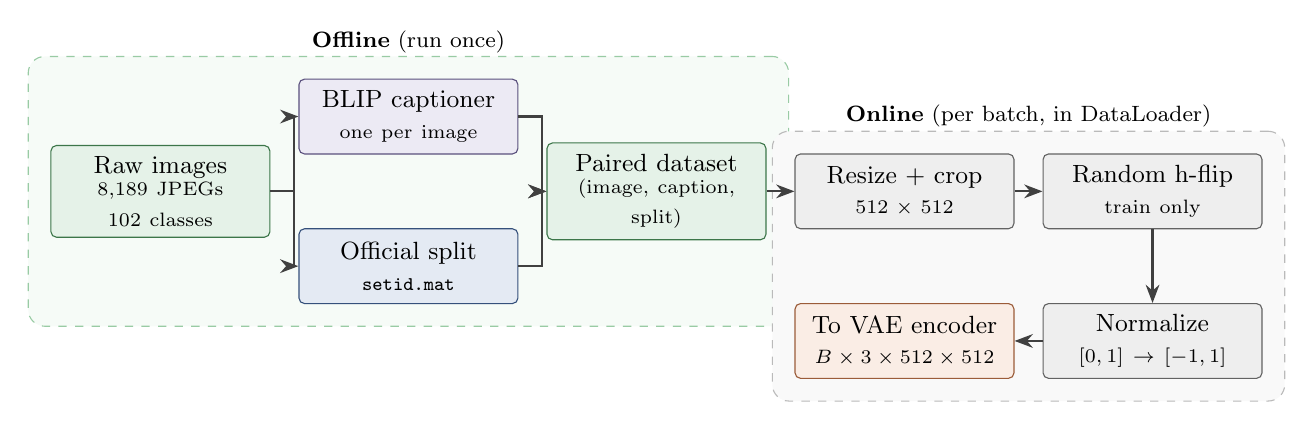
\begin{tikzpicture}[pb/.style={blk=#1, minimum height=0.95cm, text width=2.5cm}]
  % Offline stage
  \node[pb=cdata] (raw) at (0,0) {Raw images\\{\scriptsize 8,189 JPEGs\\102 classes}};
  \node[pb=ccond] (blip) at (3.15,0.95) {BLIP captioner\\{\scriptsize one per image}};
  \node[pb=cfrozen] (split) at (3.15,-0.95) {Official split\\{\scriptsize \texttt{setid.mat}}};
  \node[pb=cdata] (pairs) at (6.3,0) {Paired dataset\\{\scriptsize (image, caption,\\split)}};
  % Online stage
  \node[pb] (resize) at (9.45,0) {Resize + crop\\{\scriptsize $512\times512$}};
  \node[pb] (flip) at (12.6,0) {Random h-flip\\{\scriptsize train only}};
  \node[pb] (norm) at (12.6,-1.9) {Normalize\\{\scriptsize $[0,1]\rightarrow[-1,1]$}};
  \node[pb=ctrain] (out) at (9.45,-1.9) {To VAE encoder\\{\scriptsize $B\times3\times512\times512$}};
  \draw[flow] (raw.east) -- ++(0.3,0) |- (blip);
  \draw[flow] (raw.east) -- ++(0.3,0) |- (split);
  \draw[flow] (blip.east) -- ++(0.3,0) |- (pairs);
  \draw[flow] (split.east) -- ++(0.3,0) |- (pairs);
  \draw[flow] (pairs) -- (resize);
  \draw[flow] (resize) -- (flip);
  \draw[flow] (flip) -- (norm);
  \draw[flow] (norm) -- (out);
  \begin{scope}[on background layer]
    \node[region=cdata, fit=(raw)(blip)(split)(pairs), label={[lbl]above:\textbf{Offline} (run once)}] {};
    \node[region=cgray, fit=(resize)(flip)(norm)(out), label={[lbl]above:\textbf{Online} (per batch, in DataLoader)}] {};
  \end{scope}
\end{tikzpicture}
\caption{Data preparation pipeline. Captions and split assignments are computed once on the raw images; image transforms are applied on the fly when loading each batch.}
\label{fig:data_pipeline}
\end{figure}

\section{Results}

\subsection{Dataset Statistics}

\begin{table}[!htbp]
\centering
\caption{Final dataset composition}
\begin{tabular}{lrr}
\toprule
Split & Count & Percentage \\
\midrule
Training & 1,020 & 12.5\% \\
Validation & 1,020 & 12.5\% \\
Test & 6,149 & 75.1\% \\
\midrule
Total & 8,189 & 100\% \\
\bottomrule
\end{tabular}
\end{table}

\begin{figure}[!htbp]
\centering
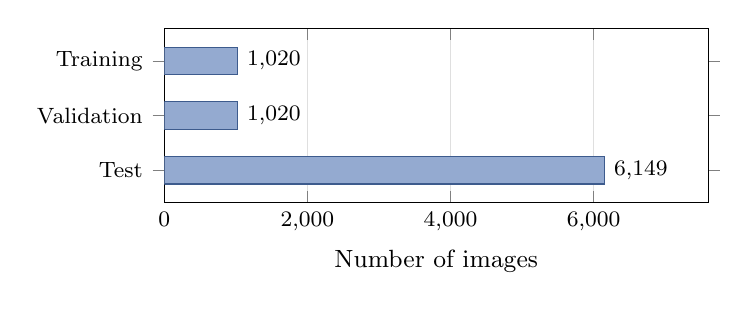
\begin{tikzpicture}
\begin{axis}[xbar, width=0.7\linewidth, height=3.8cm, xmin=0, xmax=7600,
             xlabel={Number of images}, symbolic y coords={Test,Validation,Training}, ytick=data,
             nodes near coords, nodes near coords align={horizontal},
             every node near coord/.append style={font=\footnotesize},
             bar width=10pt, enlarge y limits=0.3, ymajorgrids=false]
\addplot[fill=cfrozen!60, draw=cfrozen!80!black] coordinates {(1020,Training) (1020,Validation) (6149,Test)};
\end{axis}
\end{tikzpicture}
\caption{Official Oxford-102 split: 10 images per class for training and validation; all remaining images (20--238 per class) for testing.}
\label{fig:split}
\end{figure}

\subsection{Caption Quality}

Generated captions demonstrate semantic understanding:

\begin{itemize}
    \item Specific color descriptions (yellow, purple, blue)
    \item Structural details (petals, center, leaves)
    \item Contextual elements (garden, field, sky)
\end{itemize}

\section{Conclusion}

I prepared the Oxford-102 Flowers dataset with BLIP-generated captions and established the architectural foundations for text-to-image diffusion. The VAE compression ($48\times$) and CLIP encoding enable efficient fine-tuning while preserving semantic information. This groundwork enables the downstream contributions of training (Part 2) and evaluation (Part 3).

\begin{thebibliography}{99}

\bibitem{ho2020denoising} Ho, J., Jain, A., \& Abbeel, P. (2020). Denoising Diffusion Probabilistic Models. In Advances in Neural Information Processing Systems (NeurIPS), 33, 6840--6851.

\bibitem{rombach2021high} Rombach, R., Blattmann, A., Lorenz, D., Esser, P., \& Ommer, B. (2022). High-Resolution Image Synthesis with Latent Diffusion Models. In Proceedings of the IEEE/CVF Conference on Computer Vision and Pattern Recognition (CVPR), 10684--10695.

\bibitem{nilsback2008automated} Nilsback, M.-E., \& Zisserman, A. (2008). Automated flower classification over a large number of classes. In Sixth Indian Conference on Computer Vision, Graphics \& Image Processing (pp. 722--729). IEEE.

\bibitem{li2022blip} Li, J., Li, D., Xiong, C., \& Hoi, S. (2022). BLIP: Bootstrapping Language-Image Pre-training for Unified Vision-Language Understanding and Generation. In International Conference on Machine Learning (pp. 12888--12900). PMLR.

\bibitem{radford2021learning} Radford, A., Kim, J. W., Hallacy, C., Ramesh, A., Goh, G., Agarwal, S., et al. (2021). Learning transferable visual models from natural language supervision. In International Conference on Machine Learning (pp. 8748--8763). PMLR.

\end{thebibliography}

\end{document}
